% Tipo de documento. En este caso es un art�culo, para folios A4, tama�o de la fuente 11pt y con p�gina separada para el t�tulo
\documentclass[a4paper,12pt,titlepage]{article}

% Carga de paquetes necesarios. OrdenesArticle es un paquete personalizado
\usepackage[spanish]{babel} 
\usepackage[T1]{fontenc}
\usepackage[ansinew]{inputenx} 
\usepackage[spanish,cap,cont,title,fancy]{OrdenesArticle}
\usepackage{setspace}
\usepackage{array}
\usepackage{graphicx}
\usepackage{hyperref}
\usepackage{pifont}
\usepackage{listings}
\usepackage[usenames,dvipsnames]{color}
\usepackage{colortbl}
\usepackage{makeidx}
\hypersetup{bookmarksopen,bookmarksopenlevel=3,linktocpage,colorlinks,urlcolor=blue,citecolor=blue,
						linkcolor=blue,filecolor=blue,pdfnewwindow,
						pdftitle={Auditor�a a DIGSOL}, 
						pdfauthor={Juan Andrada, Jose Domingo L�pez, Antonio Mart�n Menor, Francisco Jos� Oteo}}


% Macro para definir una lista personalizada 
\newenvironment{milista}%
{\begin{list}{\textbullet}%
{\settowidth{\labelwidth}{\textbullet} \setlength{\leftmargin}{\dimexpr\labelsep+\labelwidth+5pt}
\setlength{\itemsep}{\dimexpr 0.5ex plus 0.25ex minus 0.25ex}
\setlength{\parsep}{\itemsep}
\setlength{\partopsep}{\itemsep}
\addtolength{\topsep}{-7.5pt}
}}%
{\end{list}}

\begin{document}

% En las p�ginas de portada e �ndices, no hay encabezado ni pie de p�gina
\pagestyle{fancy} 

% Se incluye la portada
\begin{titlepage}
	\begin{center}
  	{\LARGE UNIVERSIDAD DE CASTILLA-LA MANCHA} \\
  	\bigskip
  	{\Large ESCUELA SUPERIOR DE INFORM�TICA} \\
  	\vspace{20mm}
  	
\includegraphics[scale=0.45, keepaspectratio]{esi_bw.png} \\
  	\vspace{20mm}
  	{\Huge \textbf{Auditor�a y Seguridad de la Informaci�n}} \\
  	\vspace{10mm}
  	{\LARGE \textsc{\textbf{Auditor�a a DIGSOL}}} \\
  	\vspace{30mm}
  	\today
  	\vspace{30mm}
  	\begin{flushleft}
  		{\large Juan Andrada Romero}\\
  		\vspace{1mm}
  		{\large Jose Domingo L�pez L�pez}\\
  		\vspace{1mm}
  		{\large Antonio Mart�n Menor de Santos}\\
  		\vspace{1mm}
  		{\large Francisco Jos� Oteo Fern�ndez}\\  		
  	\end{flushleft}
	\end{center}
\end{titlepage}

% Se ajusta la separaci�n entre p�rrafos
\parskip=10pt

% Aqui se incluyen los archivos .tex que forman el documento
\section{Carta al Director}
\input{CartaDirector.tex}
\clearpage

\section{Auditor�a}
\subsection{Ausencia de un plan estrat�gico de Tecnolog�as de la Informaci�n}

\begin{spacing}{1.4}

Consultando al Comit� de Direcci�n de la empresa sobre la existencia de un plan estrat�gico de TI (Tecnolog�as de la Informaci�n), se ha observado que no existe dicho plan. Esto significa que, a la hora de intentar cumplir los objetivos de negocio que la empresa tiene fijados, las tecnolog�as no son algo importante para conseguirlos, si no una simple ayuda (ver Anexo 1).\\
\indent Es decir, la empresa no est� alineada con la tecnolog�a, lo que puede suponer, a largo o medio plazo, que la empresa comience a perder presencia en el mercado, ya que para seguir siendo competitiva, es necesario investigar nuevas tecnolog�as, actualizar los recursos tecnol�gicos con los que ya cuenta la empresa y aprovechar las oportunidades que ofrecen las tecnolog�as de la informaci�n. En el Anexo 2 se muestra la inversi�n que las empresas de la competencia realizan en I+D de nuevas tecnolog�as y la situaci�n actual en el mercado. Como se puede observar, si la empresa no alinea las tecnolog�as con su objetivo de negocio, en poco tiempo perder� la posici�n en el mercado con respecto a su competidora m�s inmediata.

Derivado de la inexistencia de un plan estrat�gico de TI que alinee las tecnolog�as con el objetivo de negocio, aparece otro problema, que es la falta de un Departamento de Sistemas de Informaci�n en la organizaci�n de la empresa, tal y como se observa en el Anexo 3. Como consecuencia, los desarrolladores inform�ticos est�n asociados a los diferentes departamentos de la empresa, desarrollando los proyectos que sean necesarios en cada momento (entre otras cosas), pero sin contar con un responsable experto en TI.

Al carecer de un Departamento de Sistemas de Informaci�n, no hay ning�n responsable que se encargue de elaborar un plan para la adquisici�n y mantenimiento de recursos tecnol�gicos (ver Anexo 1). Por ello, como la empresa carece de dicho plan, cuando cada departamento solicita nuevos recursos tecnol�gicos, el departamento de contabilidad aprueba la inversi�n, bajo la orden del Comit� de Direcci�n. Por esta raz�n, la inversi�n en tecnolog�a que realiza la empresa es m�s elevada de lo necesario, lo que puede traducirse en p�rdidas econ�micas importantes a largo plazo. Adem�s, los recursos se adquieren de diversos proveedores, lo que pone en riesgo la compatibilidad, tanto de hardware como de software. Por otra parte, como el Comit� de Direcci�n aprueba la inversi�n siempre que se solicitan nuevos recursos, existe el riesgo de que cualquier desarrollador cometa fraudes, pudiendo establecer como proveedor a uno con el que haya pactado alguna comisi�n o comprando recursos que �l desee y que sean totalmente innecesarios. En el Anexo 4 puede verse un ejemplo de estas situaciones.

Otro problema es que no existe un procedimiento por el que se sigan unas pautas a la hora de realizar pagos o devoluciones de los recursos adquiridos, as� como tampoco los contratos firmados con los proveedores han sido revisados por un asesor legal, ni se indican cl�usulas u obligaciones que deben cumplirse por parte de los proveedores (ver Anexo 1). Al no establecerse esas cl�usulas contractuales, si un proveedor no satisface un pedido en el per�odo acordado, puede repercutir en graves p�rdidas econ�micas, lo que pone en riesgo la disponibilidad de alg�n recurso y, por tanto, el correcto funcionamiento de la empresa, con las correspondientes p�rdidas econ�micas. 

Al igual que no existe un plan para la adquisici�n de infraestructura tecnol�gica, tampoco existe un plan para su mantenimiento, como muestran los Anexos 1 y 5. Simplemente, los encargados de inform�tica de cada departamento realizan las labores de mantenimiento necesarias cuando ocurre alg�n problema, al igual que se encargan de aplicar las actualizaciones necesarias al software instalado. Esto conlleva un descontrol, ya que no se relizan documentos acerca del mantenimiento realizado ni se sigue un control de cambios en el software que utiliza la empresa.

Para terminar, hay que se�alar otro problema. Al no existir el plan estrat�gico que alinee la empresa con las TI, tampoco existen portafolios de proyectos (esto es, lista de proyectos a desarrollar en la empresa) que asigne correctamente las prioridades a los diferentes proyectos que maneja la empresa. As�, los desarrolladores inform�ticos se limitan a desarrollar las aplicaciones que dichos departamentos necesiten para llevar a cabo su tarea, en el orden en el que los empleados las van solicitando (ver Anexo 5).\\
\indent Esto tiene el riesgo de que no se atiendan a tiempo los proyectos m�s prioritarios para mantener el objetivo de negocio de la empresa y que, por tanto, se produzcan p�rdidas econ�micas, adem�s de perder competitividad en el mercado.

% Como papel de trabajo, nos podemos inventar unos planes de proyecto 
% o unos calendarios donde se muestre que no se sigue un orden a la 
% hora de realizar los proyectos

\end{spacing}

%% -*- coding: utf-8 -*-

\subsection{Problemas relacionados con la Planificaci�n Estrat�gica de TI}

\begin{spacing}{1.4}

% Problemas relacionados con el objetivo de control PO1.1, PO1.2, PO1.4
Consultando al Director General sobre la existencia de un plan estrat�gico de TI, se ha observado que no existe dicho plan. Por tanto, la empresa no est� alineada con las tecnolog�as de la informaci�n, lo que puede suponer, a largo o medio plazo, que la empresa comience a perder presencia en el mercado, ya que para 
seguir siendo competitiva, es necesario investigar nuevas tecnolog�as, actualizar las que ya tiene y aprovechar las oportunidades que ofrece las tecnolog�as de la informaci�n.

Derivado de la inexistencia de un plan estrat�gico de TI que alinee las tecnolog�as con el objetivo de negocio, aparece otro problema, que es la falta de un Departamento de Sistemas de Informaci�n en la organizaci�n de la empresa. Esto provoca que, cuando cada departamento solicita nuevas tecnolog�as, la direcci�n lo aprueba, ya que no hay ning�n especialista que pueda administrar el valor de las TI actuales. Por esta raz�n, la inversi�n en tecnolog�a que realiza la empresa es m�s elevada de lo necesario, lo que puede traducirse en p�rdidas econ�micas importantes a largo plazo. 

% Problemas relacionados con el objetivo de control PO1.6
Por otra parte, como no existe un plan que coordine todo lo relacionado con las tecnolog�as de la informaci�n, no existen portafolios de proyectos que asigne correctamente las prioridades a los diferentes proyectos que maneja la empresa. As�, los desarrolladores inform�ticos (que est�n asociados a los distintos departamentos de la empresa) se limitan a desarrollar las aplicaciones que dichos departamentos necesiten para llevar a cabo su tarea, en el orden en el que se van solicitando. Esto provocar� que no se atiendan a tiempo los proyectos m�s prioritarios para mantener el objetivo de negocio de la empresa y se produzcan p�rdidas econ�micas, adem�s de perder competitividad en el mercado.

\end{spacing}




\clearpage
\subsection {Evaluaci�n de riesgos, plan de contingencia y plan de continuidad}

\begin{spacing}{1.4}

La evaluaci�n y gesti�n de riesgos es un tema que no est� abordado de
una forma eficiente en la organizaci�n.

Aunque la empresa dispone de un plan de riesgos, �ste ha sido elaborado por algunos de
los miembros del Consejo de Administraci�n y no existe ning�n informe
en el cual se indique qui�nes de estos miembros estaban presentes en la
elaboraci�n del plan ni las personas a las que consultaron a la hora
de realizarlo. 

Adem�s, tampoco existe ning�n registro de la t�cnica de
identificaci�n de riesgos que emplearon para seleccionarlos, as� como el 
c�lculo de la probabilidad de ocurrencia y el impacto, lo cual puede 
significar que la elecci�n de �stos par�metros fuese arbitraria o manipulada. 
En el Anexo 22 se muestra el acta de los asistentes a dicha reuni�n.

La empresa por tanto, no tiene definido un plan de continuidad de TI por lo que en caso de interrupci�n de los sistemas el impacto ser� mayor y en consecuencia se ver�n afectados
los procesos clave de negocio.

De lo anterior se extrae que la empresa tendr�a dificultades para volver a su actividad normal en caso de un desastre o contingencia lo que podr�a provocar perdidas muy grandes para la 
empresa.

Las copias de seguridad que posee la empresa no son suficientemente frecuentes. Adem�s carece de copias de seguridad fuera de las instalaciones por lo que en caso de desastre en las instalaciones
existe el riesgo de perder toda la informaci�n relevante de la empresa. En el Anexo 23 se muestra c�mo se almacenan algunas de las copias de seguridad.

\end{spacing}
%% -*- coding: utf-8 -*-

\subsection{Problemas relacionados con la Arquitectura de la Informaci�n}

\begin{spacing}{1.4}

%En cuanto a diccionario de datos empresarial y reglas de sintaxis

La empresa DIGSOL carece de un diccionario de datos empresarial que defina las reglas
de sintaxis para los datos de la organizaci�n lo que produce:
-Peor entendimiento entre los usuarios del sistema de TI y del Negocio.
-Posibilidad de creaci�n de elementos de datos incompatibles.

%En cuanto al esquema de clasificacion de datos y la administraci�n de la integridad
Existe un esquema de clasificaci�n de datos definido en el que cada tipo de usuario tiene
acceso a una informaci�n concreta pero al no encriptar la informaci�n que viaja en texto plano
por la red local es f�cilmente interceptable por los dem�s usuarios de la empresa incluso por usuarios
externos ya que adem�s la protecci�n de la wifi se realiza mediante clave WEP que es un tipo de clave 
f�cil de obtener mediante aplicaciones como AirCrack lo que compromete la integridad del sistema.

Los USB y los dispositivos �pticos de los ordenadores de la empresa no 
est�n bloqueados, lo que permitir�a que un usuario malintencionado tomar documentos
 y datos de car�cter confidencial para la empresa, introducir virus o troyanos en el sistema.
%En cuanto a Administraci�n de integridad

No existen procedimientos peri�dicos para cambio de contrase�as de los
usuarios en el sistema. Estas claves son facilitadas en la incorporaci�n del
usuario a la empresa y no son eliminadas tras su despido por el departamento de
SI cuando recibe la confirmaci�n pertinente.

El diagrama de la base de datos es correcto pero su implementaci�n no es coherente con el diagrama dise�ado.
Una vez hemos estudiado la base de datos hemos comprobado que las claves ajenas est�n ausente en la creaci�n 
de las tablas, as� como campos que no deben estar vacios est�n definidos con la posibilidad de serlo.

El acceso a la base de datos es posible si se conoce la cadena de conexi�n a la misma ya que carece de clave de
usuario y de acceso ya que se ha utilizado SQL Server con modo de autenticaci�n de Windows. Es posible obtener 
la ruta de acceso a la base de datos utilizando aplicaciones sniffer que se utilizan para escuchar la 
informaci�n que viaja por nuestra red local de forma que podemos obtener m�s informaci�n de la que el usuario
debiese obtener.

Carece de una base de datos centralizada que contenga la informaci�n completa de la empresa, hay una base de datos
que almacena una parte (productos,empleados,usuarios registrados...) y otra parte que se almacena en ficheros de texto
como facturas... Puesto que las facturas est�n relacionadas con productos, usuarios registrados y empleados entre otros
estas deber�an estar integradas en la base de datos centralizada.



\end{spacing}


\clearpage
%La evaluación y gestión de riesgos es un tema que no está abordado de
una forma eficiente en la organización ya que, aunque la empresa
dispone de un plan de riesgos, éste ha sido elaborado por algunos de
los miembros del Consejo de Administración y no existe ningún informe
en el cual se indique quiénes de estos miembros estaban presentes en la
elaboración del plan ni las personas a las que consultaron a la hora
de realizarlo. Además, tampoco existe ningún registro de la técnica de
identificación de riesgos que emplearon (p.e. Delphi) para
seleccionarlos, lo cual puede significar que la elección de éstos
fuese arbitraria o manipulada. En el Anexo ?? se muestra el acta de
los asistentes a dicha reunión. 

Un aspecto a destacar en los riesgos seleccionados y planificados es
que se ciñen al ámbito software dejándo de lado el ámbito hardware, no
teniendo en  cuenta, por ejemplo, factores externos sobre los cuales
la organización puede no tener ningún control debido a su naturaleza
(terremotos, colisiones de aviones, etc...) o incluso el robo de material o
incendios. En el Anexo ?? se puede observar una lista de los riesgos
que deberían ser revisados y/o considerados.

Además, el CIO y el Consejo de Administración han ido elaborando una
lista de los nuevos riesgos que han ido azotando a la organización
pero no los han documentado en términos del impacto que éstos
produjeron ni las estrategias de mitigación o planes de contigencia
que se llevaron a cabo para combatirlos con el objetivo de reutilizarlos
o de mejorarlos. Debido a ésto, algunos riesgos se han producido
en varias ocasiones y no se ha ido reduciendo el impacto. Como prueba
de ello, en el Anexo ?? se puede apreciar que la empresa ha sufrido
dos apagones de luz generales en seis meses, las pérdidas económicas
que supusieron ámbos, el coste de haber desarrollado un plan de
contigencia, y las pérdidas que se habrían producido si dicho plan se
hubiese llevado a cabo.


\subsection {Gesti�n de la configuraci�n y control de cambios}

\begin{spacing}{1.4}

La empresa dispone de una herramienta de soporte y un repositorio central para almacenar informaci�n relevante sobre los elementos de configuraci�n hardware y software. El objetivo es garantizar la integridad de las configuraciones, pero este repositorio no se encuentra actualizado con las nuevas adquisiciones y necesidades de la empresa, ni con la evoluci�n de las TI.

En el \textbf{Anexo 6} se observa un fragmento un documento, proporcionado por el Gerente de configuraci�n, que especifica la configuraci�n inicial de los equipos que utilizar�n los empleados. Como se puede apreciar, el software que inicialmente se instalar� en estos equipos est� obsoleto y no existe una norma que est�ndarice la instalaci�n de parches y actualizaciones de seguridad, as� como la configuraci�n de servicios y par�metros del sistema. Esto hace que los sistemas no sean seguros y sean cada vez m�s vulnerables a ataques inform�ticos (\textbf{ver Anexo 7}, proporcionado por el Jefe de Seguridad).

Otra de las consecuencias que acarrea no tener actualizado el repositorio afecta al uso y adquisici�n de licencias. En el \textbf{Anexo 8} se puede apreciar que en el �ltimo a�o se han adquirido licencias duplicadas para el antivirus y que a�n as� existen equipos con licencias caducadas \textbf{(ver Anexo 9)}. Este problema, cuantificando �nicamenten el caso del antivirus, ha supuesto un total de 676 euros adicionales en 6 meses, un gasto totalmente innecesario.

Por otro lado, los cambios realizados no son registrados en ning�n documento y no se mantiene una l�nea base de los elementos de la configuraci�n para todos los sistemas y servicios como punto de comprobaci�n al que volver tras el cambio. Adem�s, no se garantizan los resultados de los cambios antes de realizarse, ya que �stos no est�n sujetos a ning�n tipo de norma y cada usuario los hace libremente. Como prueba de ello, en el \textbf{Anexo 10} se observan capturas de pantalla de software personal, no licenciado o no alineado con el negocio de la empresa y que ha sido instalado en los equipos. Esto podr�a haberse corregido si los equipos se hubiesen sido revisados peri�dicamente por el Gerente de configuraci�n.

\end{spacing}
\clearpage
%% -*- coding: utf-8 -*-

\subsection{Problemas relacionados con Adquirir y Mantener Infraestructura Tecnol�gica}

\begin{spacing}{1.4}

% Relacionado con el punto AI3.1
Como ya se ha comentado, la empresa carece de un Departamento de Sistemas de Informaci�n que pueda, entre otras cosas, elaborar un plan para la adquisici�n y mantenimiento de recursos tecnol�gicos. Por ello, cuando cada departamento solicita nuevas tecnolog�as, la direcci�n lo aprueba, ya que no hay ning�n responsable que pueda evaluar si realmente la adquisici�n de hardware es necesaria. Por esta raz�n, la inversi�n en tecnolog�a que realiza la empresa es m�s elevada de lo necesario, lo que puede traducirse en p�rdidas econ�micas importantes a largo plazo. En el Anexo ?? (p�gina \pageref{anexo:facturas}) puede verse un ejemplo de gastos innecesarios en tecnolog�as.

Adem�s, tampoco se realiza un seguimiento ni una evaluaci�n para comprobar que los nuevos recursos obtenidos (principalmete hardware) est�n aportando beneficio a la empresa y est�n ayudando a cumplir su objetivo de negocio. 

\end{spacing}
% -*- coding: utf-8 -*-

\subsection{Deficiencia en la seguridad de la informaci�n y en las instalaciones}

\begin{spacing}{1.4}

Continuando con la auditor�a, con respecto a las instalaciones de la empresa, se observa que:
	- Las instalaciones son poco o nada seguras.
	- Existen deficiencias en la ubicaci�n del servidor.
	
	Observando el entorno de trabajo y las instalaciones que posee la empresa se ve que carece de cualquier tipo de medida sobre la restricci�n o no del acceso a las instalaciones por parte del personal como por parte de personal ajeno a la empresa.
	Todas las salas en las que se ubican los departamentos carecen de cerraduras en las puertas o de sistemas de acceso controlado, tampoco se controla el acceso a la empresa de ninguna manera. Cualquiera puede entrar a las instalaciones de la empresa y acceder a cada departamento pudiendo llevarse f�sicamente cualquier dispositivo que contenga informaci�n, lo que provoca un grave riesgo en la seguridad.
	Cuando se pregunta si exist�a y se pod�a revisar el plan de seguridad con las medidas relativas al acceso a las instalaciones se obtuvo una respuesta negativa.
	
	La ubicaci�n del centro de datos y del servidor que los contiene no ha sido bien planeada y estudiada ya que no se corresponde con el dise�o �ptimo que debe tener el espacio f�sico destinado a servidores, por lo que existe riesgo de que el servidor se caliente en exceso y se estropee dejando sin servicio de venta online a la empresa, lo que se traducir�a en cuantiosas p�rdidas econ�micas, tanto en ventas como en deterioro de la imagen de la empresa en internet.	
En caso de incendio, inundaci�n o alg�n otro desastre, el servidor que contiene los datos podr�a estropearse, ya que, como se ha observado, el local en el que se ubica no es el apropiado ni est� dotado de medidas de prevenci�n y protecci�n ante tales eventualidades.

	Finalmente hay que destacar que no existe ning�n sistema de alimentaci�n ininterrumpida ni tampoco una fuente de corriente alternativa, por lo que cualquier corte de luz llevar�a forzosamente a una suspensi�n del servicio de venta por internet as� como del acceso a datos de otra �ndole, por no hablar de posibles da�os en el servidor y p�rdida de datos.
	
Con respecto a medidas de seguridad f�sicas para limitar o impedir el acceso a dispositivos y a la informaci�n que estos contienen se puede observar que el servidor no se encuentra dentro de un armario de datos bajo llave, sino que se encuentra en una estanter�a junto con otros ordenadores.
	Tanto las ranuras de expansi�n USB, como la grabadora de DVD que contiene el servidor est�n visibles y accesibles, pero adem�s, la parte posterior del servidor est� tambi�n accesible y pueden observarse las tarjetas de red. Si alg�n empleado malintencionado quisiera llevarse datos podr�a hacerlo pinchando una memoria USB, grabando un DVD o conectando otro PC a una tarjeta de red del servidor, interrumpiendo adem�s el servicio web o de acceso a los datos. \textbf{(Ver anexo 14)}.
	
	La ausencia de un cortafuegos f�sico que limite el acceso al mismo desde fuera es otra deficiencia de la seguridad importante, ya que puede dar lugar a que datos de car�cter personal sobre los empleados de la empresa, cuentas, claves, etc. pueden ser accedidos desde fuera de la empresa v�a web.
	
Cuando se pregunt� al personal responsable de inform�tica sobre qu� procedimientos se segu�an para el correcto procesamiento y almacenamiento de los datos de la empresa se nos contest� que s� se hab�a definido un responsable para administrar esos datos y su almacenamiento, pero que no se le hab�a informado sobre la existencia de ning�n procedimiento, por lo que se hab�a optado por almacenar todos los datos en un mismo servidor, incluso en un mismo directorio dentro de �ste.
Indagando un poco m�s se descubri� que s� se realizaban copias de seguridad de los datos, tanto los referidos a la informaci�n sensible a la empresa, como la informaci�n de los productos que venden; lamentablemente el soporte en el que se almacena la copia de respaldo de esos datos es un disco duro externo que se guarda en un caj�n, sin vigilancia ni medidas de seguridad, del mismo edificio en el que se encuentra el servidor. \textbf{(Ver anexo 15)}.

	A parte del encargado de administrar los datos, nadie accede, en principio, a los datos, pero no se toman las medidas de seguridad apropiadas para asegurarse de que no accedan a los datos personas no autorizadas. De hecho se ha preguntado por los ficheros de \textit{log}, pero examinando los logs de accesos al sistema se ha detectado que existen accesos al servidor por empleados que usan la cuenta -empleado- y no est�n relacionados con datos inform�ticos, incluso puede que alguno de esos accesos se hayan hecho por empleados que fueron despedidos, pero no se puede probar ya que todos los empleados usan la misma cuenta. Se advierte de que la informaci�n que dichos usuarios puedan extraer de la empresa podr�a ser vendida a la competencia. Adem�s, dichos logs corresponden �nicamente a los �ltimos 3 meses de actividad, siendo de 2 a�os el periodo exigido por la ley. \textbf{(Ver anexo 16)}.

	Respecto a ficheros de datos, cuyo soporte no es el electr�nico, se encuentra una estanter�a llena de papeles con informaci�n relevante para la empresa. Esta estanter�a no est� protegida bajo llave u otros sistemas de seguridad, y adem�s mezcla datos y cajas u otras cosas sin un orden aparente. Aqu� existe tambi�n un serio problema de seguridad, ya que la informaci�n contenida en esos papeles puede ser f�cilmente accedida. \textbf{(Ver anexo 17)}.
	
	Estudiando los comportamientos de seguridad de los empleados se observa que:
		- El estado de sus ordenadores no es el adecuado. Tienen los ordenadores abiertos f�sicamente, dejando al descubierto la electr�nica y los dispositivos de almacenamiento de datos (como el disco duro), siendo relativamente f�cil da�ar un equipo o robar informaci�n del mismo. \textbf{(Ver anexo 18)}.
		- Por otro lado, cuando un empleado abandona su puesto de trabajo, �ste no bloquea el acceso al mismo, por lo que cualquier otro empleado podr�a usar este ordenador con fines malintencionados. \textbf{(Ver anexo 21)}.

	A la hora de eliminar o destruir datos existen dos v�as para hacerlo: si los datos se encuentran en soporte electr�nico, es el administrador de datos el que los borra; y, si los datos est�n en papel, para eliminarlos se rompe el papel y se tira a la papelera. En cuanto al procedimiento a seguir cuando se estropea un soporte de almacenamiento, no est� especificado, por lo que simplemente, o bien se tira a la basura o bien se lleva a reciclar, pero no se destruye la informaci�n que contiene, por lo que alguien podr�a recuperar esos datos de alguna manera usando un lector magn�tico, etc. \textbf{(Ver anexos 19 y 20)}.
	
	Tampoco se han encontrado existencias de un libro de incidencias, tal y como dicta el art�culo 10 del Real Decreto 994/99, en que hagan constar los siguientes puntos:
		a) el tipo de incidencia
		b) El momento en que se produce
		c) La persona que realiza la notificaci�n
		d) A qui�n se le comunica
		e) Los efectos que se deriven de la incidencia.

\end{spacing}
\clearpage
%% -*- coding: utf-8 -*-

\subsection{Problemas relacionados con la adquisici�n de recursos de TI}

\begin{spacing}{1.4}
Al realizar la auditor�a nos hemos fijado en estas �reas dentro de la compa��a: infraestructura hardware, software y la seguridad de los datos.
Respecto a la infraestructura hardware de la empresa, y m�s concretamente, el proceso de adquisici�n de hardware se ha detectado que ni existe ni est� definida una pol�tic a seguir a la hora de adquirir nuevos dispositivos hardware.
Este es, claramente, un riesgo para el TI ya que no se controla qui�n realiza la adquisici�n de hardware, ni si previamente alguien le ha dado una lista de dispositivos que se deben adquirir, etc. No se especif�ca en ning�n documento qui�n es el responsable del desarrollo de unos procedimientos a seguir a la hora de adquirir nuevos dispositivos, existe una lista de proveedores, pero no se ind�ca qui�n estableci� esalista ni qui�n debe actualizarla.
Tampoco se indica si se consulta o no al CEO y al CFO, por lo que existe el riesgo de que cualquier empleado cometa fraudes pudiendo establecer como proveedor a uno con el que haya pactado pero cuyos precios no se ajusten a la pol�tica de gastos o precios de la empresa.
Con respecto a la adquisici�n del software si existen unas pol�ticas definidas. Una vez revisadas se observan algunos riesgos como son la ausencia de un responsable claro que rinda cuentas sobre qu� lista de proveedores se ha hecho y c�mo se mantiene esta (acualiz�ndola a�adiendo o eliminando proveedores).
Una vez que se realiza un pedido, ya sea de hardware o de software, no existe un procedimiento por el que se sigan unas pautas a la hora de realizar pagos o devoluciones; tampoco se indican cl�usulas  u obligaciones que deben cumplirse por parte de los proveedores. Adem�s otro riesgo detectado es que ninguno de los contratos firmados con los proveedores ha sido revisado por un asesor legal.
Al no establecerse esas clausulas contractuales, si un proveedor no satisface un pedido en el periodo acordado puede repercutir en graves p�rdidas econ�micas, debido a que la empresa vende productos por internet y la no disponibilidad de un producto haga que se pierda su venta y que la credibilidad y seriedad de la empresa vea da�ada su imagen.

\end{spacing}
\subsection{Integridad, disponibilidad y confidencialidad de los datos}

\begin{spacing}{1.4}

La empresa carece de servidor de respaldo donde se almacenen duplicados todos los datos de la empresa. Esto indica que existir�a un problema serio de disponibilidad de los datos ante una posible aver�a en el servidor principal, o ante un desastre, provocando una interrupci�n en el servicio de venta online y por lo tanto la falta de continuidad del negocio.

Otro punto d�bil que se ha encontrado es la existencia de una �nica cuenta de usuario dentro del servidor que sirve de puerta de acceso a �ste y a los datos que contiene, tanto para los empleados de la empresa relacionados con la parte inform�tica de cada departamento, como para el administrador del servidor. Esta cuenta se llama igual que el nombre de la empresa y el servidor, por lo que ser�a f�cil adivinar desde fuera cu�l podr�a ser un usuario del sistema y lanzar un ataque contra �l. \textbf{(ver anexo 11)}. \\
\indent Adem�s, si un empleado con alg�n conocimiento de administraci�n quisiese modificar datos de los archivos, no tendr�a grandes problemas, debido a que varios archivos tienen permisos de lectura y escritura para el grupo de usuarios al que pertenece el usuario \textit{empleado} y el usuario \textit{digsol}. \textbf{(ver anexos 11 y 12)}.

Otro problema es el hecho de que se use el servidor tanto para almacenar los datos referidos a los productos que se venden en la web, como datos sensibles sobre la empresa, referidos a la informaci�n de car�cter personal sobre empleados, clientes, n�minas, etc.
Ciertos archivos con informaci�n de car�cter personal y/o confidencial tienen unos permisos inadecuados, lo que evidencia un gran riesgo ya que cualquiera (ya sea o no usuario del sistema) puede tener acceso a esta informaci�n y leerla, modificarla o borrarla. Incluso existen ficheros en texto plano y sin cifrar que contienen las claves de acceso al sistema. Esto repercute tanto en la confidencialidad de los datos como en la integridad y disponibilidad de los mismos. \textbf{(ver anexo 12)}.

Al consultar al administrador del servidor sobre la administraci�n y gesti�n de cuentas de usuario y sobre si existe una pol�tica definida a tal efecto, �ste ha comunicado que no existe una pol�tica que obligue a los usuarios del sistema a cambiar su contrase�a personal en un per�odo definido de tiempo, no pudiendo ser �sta la misma que una contrase�a anterior. Esto hace que si un usuario no autorizado consigue acceso mediante alguna cuenta, podr� hacerlo de por vida ya que la contrase�a no ser� modificada en un futuro pr�ximo.

Al igual que no existe un plan para la administraci�n de los datos, tampoco existe un plan para su mantenimiento. Simplemente, el encargado del servidor se encarga de dar de alta a los usuarios del sistema y asignarles claves; pero a su vez tambi�n se encarga de actualizar los datos de la web de venta de art�culos. Igualmente, los encargados de inform�tica de cada departamento tienen acceso al servidor usando una �nica cuenta (como ya se ha comentado) y realizan las labores de mantenimiento necesarias con los datos y los archivos que los contienen, al igual que se encargan de aplicar las actualizaciones necesarias al software instalado. \\
\indent Esto conlleva un serio riesgo de integridad y seguridad de los datos, ya que cualquier trabajador podr�a alterar archivos de datos sin ning�n tipo de control sobre �l.

No se han creado planes para poder monitorear el desempe�o de las tecnolog�as de informaci�n ni para medir su capacidad. Puntualmente, los desarrolladores inform�ticos revisan los recursos para comprobar si pueden soportar la carga de trabajo de los distintos departamentos. Sin embargo, dichas revisiones no se documentan y las acciones tomadas se limitan a solicitar nuevos recursos tecnol�gicos si se observa que los actuales no soportan correctamente la carga de negocio. \\
\indent Por tanto, no se monitorea la capacidad actual de los recursos, as� como tampoco se tiene en cuenta el posible crecimiento futuro de la empresa, lo que supondr� un aumento en la carga de trabajo, existiendo un riesgo que pone en peligro la disponibilidad de los recursos.

Respecto a los diccionarios de datos que utiliza la empresa, la empresa carece de un diccionario de datos empresarial que defina las reglas de sintaxis para los datos de la organizaci�n, lo que produce un peor entendimiento entre los usuarios del sistema y del negocio y la posibilidad de creaci�n de elementos de datos incompatibles, por lo que existe un riesgo ante la integridad de los datos.

Otro punto d�bil que afecta a la integridad de los datos es el hecho de que las comunicaciones por la red no est�n cifradas por lo que, al no encriptar la informaci�n (que viaja en texto plano por la red local), es f�cilmente interceptable por los dem�s usuarios de la empresa o incluso por usuarios externos, ya que adem�s la protecci�n de la wifi se realiza mediante clave WEP que es un tipo de clave f�cil de obtener mediante aplicaciones como AirCrack, lo que compromete la integridad del sistema. \textbf{(ver anexo 13)}.

Para terminar, existe un riesgo para la integridad de la informaci�n, ya que se carece de una base de datos centralizada que contenga la informaci�n completa de la empresa. Hay una base de datos que almacena una parte de los datos (productos, datos de clientes, etc.) y otra parte que se almacena en ficheros de texto (facturas, etc.) o en ficheros de bases de datos Access o Excel. Puesto que las facturas est�n relacionadas con productos, usuarios registrados y empleados entre otros, estas deber�an estar integradas en una base de datos centralizada, y no repartidos por diferentes ubicaciones. \textbf{(ver anexo 12)}.

\end{spacing}

\clearpage
%% -*- coding: utf-8 -*-

\subsection{Problemas relacionados con los cambios}

\begin{spacing}{1.4}

La empresa carece de procediminetos de administraci�n de cambios formales para manejar de manera est�ndar todas las solicitudes que afectan a:
\begin{enumerate}
	 \item Cambios de aplicaciones software.
	 \item Cambios de procedimientos.
	 \item Cambios de procesos.
	 \item Cambios de par�metros del sistema.
	 \item Cambios de par�metros de servicio.
	 \item Cambios de las plataformas fundamentales.
\end{enumerate}

Del mismo modo, los cambios realizados no son registrados en ning�n sitio ni previamente autorizados. Adem�s, no se garantizan los resultados de los cambios antes de realizarse
ya que no existe ning�n metodo de evaluaci�n de los impactos de los cambios en el sistema operacional y su funcionalidad. 

La empresa tambi�n carece de un plan de cambios de emergencia que defina, plantee, evalue y autorice los posibles cambios de emergencia.

Con respecto a los cambios aplicados no existe un sistema de seguimiento y reporte de los mismos que mantengan informados a los solicitantes del cambio y a los interesados
relevantes, acerca del estado de cambio de las aplicaciones, procedimientos, procesos, par�metros del sistema y del servicio y de las plataformas fundamentales.

En consecuencia con todo lo anterior, se carece de un proceso de revisi�n que garantice la implantaci�n corrrecta y completa de los cambios.

Podr�amos decir que la empresa se encuentra en un nivel de madurez inicial. Se reconoce que los cambios se deben administrar y controlar pero no toman medidas.
\end{spacing}
%\clearpage
%% -*- coding: utf-8 -*-

\subsection{Problemas relacionados con Administrar el Desempe�o y la Capacidad}

\begin{spacing}{1.4}

\end{spacing}
%\clearpage
%% -*- coding: utf-8 -*-

\subsection{Problemas relacionados con la continudidad del servicio}

\begin{spacing}{1.4}

%Marco de trabajo de continuidad de TI
La empresa carece de un marco de trabajo de continuidad de TI que de soporte a la continuidad del negocio. Esto es, no se tiene un plan de recuperaci�n de desastres y
de contingencias.

%Planes de continuidad
La empresa por tanto, no tiene definido un plan de continuidad de TI por lo que en caso de interrupci�n de los sistemas el impacto ser� mayor y en consecuencia se ver�n afectados
los procesos clave de negocio.

%Recuperaci�n y Reanudaci�n
De lo anterior se extrae que la empresa tendr�a dificultades para volver a su actividad normal en caso de un desastre o contingencia lo que podr�a provocar perdidas muy grandes para la 
empresa.

%Respaldo
Las copias de seguridad que posee la empresa no son suficientemente frecuentes. Adem�s carece de copias de seguridad fuera de las instalaciones por lo que en caso de desastre en las instalaciones
existe el riesgo de perder toda la informaci�n relevante de la empresa.


\end{spacing}
%\clearpage
%Garantizar la seguridad de los sitemas

La seguridad de los sistemas se ha auditado desde el punto de vista del personal, 
del software y del hardware, y ser�n detallados a continuaci�n.

Para empezar, las licencias del antivirus y firewall utilizados por la empresa est�n 
caducadas no siendo posible actualizar las bases de datos de dichas aplicaciones, y 
las actualizaciones cr�ticas del sistema operativo empleado, Windows XP Professional, 
no han sido instaladas (ver Anexo ??). Esto expone a los computadores de la empresa 
a numerosos ataques realizados por hackers.

En cuanto a la administraci�n y gesti�n de cuentas de usuario, no 
existe una pol�tica que obligue a los usuarios del sistema a cambiar su 
contrase�a personal en un periodo definido de tiempo, no pudiendo ser �sta la 
misma que una contrase�a anterior. Esto hace que si un usuario no autorizado 
consigue acceso mediante alguna cuenta, podr� hacerlo de por vida ya que la 
contrase�a no ser� modificada en un futuro pr�ximo.

Adem�s, el sistema no proporciona un m�todo para que los usuarios puedan 
modificar su contrase�a, por lo que �stos est�n enviando correos electr�nicos 
al administrador notificando su login y el nuevo password que desean, no est�ndo 
�ste sujeto a una pol�tica que defina a qu� restricciones est� sometido (longitud 
m�nima de caracteres, uso de d�gitos, etc). Esto acarrea serios problemas ya que 
la contrase�a de cada usuario no es conocida por una �nica persona y dicho correo 
electr�nico puede ser interceptado por alg�n tercero indeseado. No terminando aqu�, 
las contrase�as se encuentran almacenadas en la base de datos en texto plano, 
de modo que cualquier persona que tenga acceso a �sta (p.e. el administrador de 
bases de datos) puede conocer la contrase�a de cualquier usuario.

Tambi�n existe una falta en cuanto la recolecci�n de cuentas basura. Actualmente 
el plan de seguridad define que el d�a 2 de Enero de cada a�o se proceder� a 
eliminar del sistema todas las cuentas de aquellos usuarios que no permanezcan en 
la empresa. Esto supone un serio problema ya que examinando los logs de accesos 
al sistema se ha detectado que un 3% �stos son de usuarios que ya no pertenecen 
a la plantilla de la empresa. Se advierte de que la informaci�n que dichos usuarios 
puedan extraer de la empresa podr�a ser vendida a la competencia. Adem�s, 
dichos logs corresponden �nicamente a los �ltimos 3 meses de actividad (ver Anexo 
?? -logs-), siendo 2 a�os lo que exige la ley.

A nivel f�sico, se han encontrado importantes vol�menes de informaci�n de 
car�cter privado y que no est�n debidamente protegidos y restringidos �nicamente 
a personal autorizado (ver Anexo ?? -foto de documentos o servidores fuera de 
un armario sin llave-), incluso partes de estos vol�menes desechados en los 
contenedores de la empresa sin haber sido destruidos previamente (ver Anexo ?? 
-foto de curriculos y cds sin destruir en un contenedor-).

Tampoco se han encontrado existencias de un libro de incidencias, tal y como 
dicta el art�culo 10 del Real Decreto 994/99, en que hagan constar los 
siguientes puntos:
a) el tipo de incidencia
b) El momento en que se produce
c) La persona que realiza la notificaci�n
d) A qui�n se le comunica
e) Los efectos que se deriven de la incidencia.

En el contexto del personal se ha detectado que algunos empleados se autentican 
en el sistema por medio de unas tarjetas con chip y que �stos se las dejan 
olvidadas cerca de su estaci�n de trabajo haciendo posible que cualquier 
persona pueda suplantar su identidad (ver Anexo ??).
%\clearpage
%Administrar la configuraci�n

La empresa dispone de una herramienta de soporte y un repositorio central para 
almacenar informaci�n relevante sobre los elementos de configuraci�n pero no se 
encuentra actualizado con las nuevas necesidades y adquisiciones de la empresa, 
es decir, inicialmente se grabaron todos los activos pero no se han ido grabando 
los cambios que �stos han sufrido. Un claro ejemplo de esta falta es la existencia 
de licencias caducadas de aplicaciones y que a�n se est�n instalando en nuevas 
computadoras. Este descontrol ha llevado a la empresa a re-adquirir 
licencias que ya pose�a y gastar un dinero innecesario (ver Anexo ??).

Por otro lado, no existe un prodecimiento que defina qu� software debe ser instalado 
en una m�quina cuando es introducida en la empresa. Esta labor la llevan a cabo 
dos t�cnicos que van instalando aplicaciones en los ordenadores conforme los usuarios 
las van necesitando y sin crear ning�n tipo de informe sobre los cambios que van 
haciendo a cada computadora.

Adem�s, se ha encontrado software personal y/o no licenciado (ver Anexo ?? -lista
de programas-) instalado en las computadoras de los empleados. Se le ha pedido 
al responsable en cuesti�n los informes de las revisiones pertinentes que se han 
llevado a cabo en dicho �mbito y no hemos obtenido respuesta alguna.


%\clearpage
%% -*- coding: utf-8 -*-

\subsection{Problemas relacionados con la administraci�n de los datos}

\begin{spacing}{1.4}
Continuando con la auditor�a, hemos observado que, con respecto a la web con la que la empresa realiza su expansi�n de negodio de venta por internet, los datos que se requieren a la hora de realizar una b�squeda son devueltos con bastante rapidez y exactitud, pero una gran deficiencia que cabe destacar es el hecho de que tanto los datos referidos a la informaci�n de los productos que se venden en la web como la informaci�n relevante de la empresa se almacenan en el mismo servidor.
Esto puede dar lugar a que datos de caracter personal sobre los empleados de la empresa pueden ser accedidos desde fuera de la empresa v�a web.
Cuando se pregunt� al personal a cargo del almacenamiento y seguridad de los datos sobre qu� procedimientos se segu�an para el correcto procesamiento y almacenamiento de los datos de la empresa se nos contest� que s� se hab�a definido un responsable para administrar esos datos y su almacenamiento, pero que no se le hab�a informado sobre la existencia de ning�n procedimiento, por lo que se hab�a optado por almacenar todos los datos en un mismo servidor, incluso en un mismo directorio dentro de �ste.
Otro fallo que encontramos, en �ste �mbito, dentro de la empresa fu� que no se hab�a adquirido un segundo servidor para replicar los datos y servicios relativos a la venta de art�culos por internet por lo que, en caso de un fallo en el primer y �nico servidor, el servicio de venta en la web quedar�a interrumpido durante horas o d�as...
Indagando un poco m�s se descubri� que s� se realizaban copias de seguridad de los datos, tanto los referidos a la informaci�n sensible a la empresa como la informaci�n de los producctos que venden; lamentablemente el soporte en el que se almacena la copia de respaldo de esos datos es un disco duro externo que se guarda en un caj�n, sin vigilancia ni medidas de seguridad, del mismo edificio en el que se encuentra el servidor.
A parte del encargado de administrar los datos, nadie accede, en principio, a los datos, pero no se toman las medidas de seguridad apropiadas para asegurarse de que no accedan a los datos personas no autorizadas.
A la hora de eliminar o destruir datos existen dos v�as para hacerlo: si los datos se encuentran en soporte electr�nico, es el administrador de datos el que los borra; y, si los datos est�n en papel, para eliminarlos se rompe el papel y se tira a la papelera. En cuanto al procedimiento a seguir cuando se estropea un soporte de almacenamiento, no est� especificado, por lo que simplemente, o bien se tira a la basura o bien se lleva a reciclar, pero no se destruye la informaci�n que contiene, por lo que algui�n podr�a recuperar esos datos de alguna manera usando un lector magn�tico...
\end{spacing}
%\clearpage
%% -*- coding: utf-8 -*-

\subsection{Problemas relacionados con el ambiente f�sico y su administraci�n}

\begin{spacing}{1.4}
Observando el entorno de trabajo y las instalaciones que posee la empresa vemos que a simple vista se carece de cualquier tipo de medida sobre la restricci�n o no del acceso a las instalaciones por parte del personal como por parte de personal ajeno a la empresa.
Cuando hemos pereguntado si exist�a y pod�amos revisar el plan de seguridad con las medidas relativas al acceso a las instalaciones se nos ha respondido negativamente. Es necesario detallar unas medidas de seguridad a tomar xa evitar el riesgo de que alguien acceda a equipos o informaci�n delicada...
Un punto d�bil que hemos encontrado relacionado con medidas de seguridad f�sica es la ausencia de un cortafuegos f�sico que impida el acceso al servidor desde el exterior de manera malintencionada pudiendo existir el riesgo de ataques que repercutan en la denegaci�n del servicio, etc.
Hemos observado que la elecci�n del centro de datos en el que tienen el servidor no se corresponde con el dise�o �ptimo que debe tener el espacio f�sico destinado a servidores, por lo que existe riesgo de que el servidor se caliente en exceso y se estropee dejando sin servicio de venta online a la empresa, lo que se traducir�a en cuantiosas p�rdidas econ�micas, tanto en ventas como en deterioro de la imagen de la empresa en internet.
En caso de incendio, inundaci�n o alg�n otro desastre, el servidor que contiene los datos podr�a estropearse, ya que, como hemos observado, el local en el que se ubica no es el apropiado ni est� dotado de medidas de prevenci�n y protecci�n ante tales eventualidades.
Finalmente descubrimos que no existe ning�n sistema de alimentaci�n ininterrumpida ni tampoco una fuente de corriente alternativa, por lo que cualquier corte de luz llevar�a forzosamente a una suspensi�n del servicio de venta por internet as� como del acceso a datos de otra �ndole, por no hablar de posibles da�os en el servidor y p�rdida de datos.
\end{spacing}
%\clearpage

\section{Papeles de Trabajo}
% Los anexos no tienen numeracion de seccion
\titleformat{\subsection}
	{\bfseries\large}
	{}
	{0.5pt}
	{}


\subsection{ANEXO 1: Situaci�n actual de las empresas competidoras} \label{anexo:graficos}

Los gr�ficos de las Figuras \ref{fig:inversion} y \ref{fig:presencia} han sido obtenidos de ?????.

\begin{figure}[!ht]
\centering
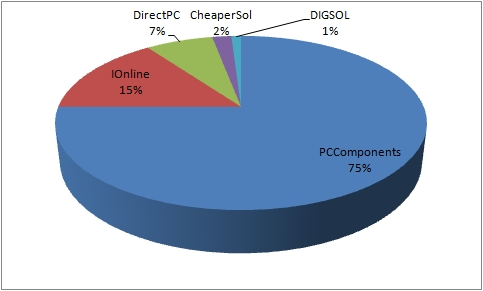
\includegraphics[scale=0.7,keepaspectratio]{./images/investigacion}%
\caption{Porcentaje de inversi�n en investigaci�n de nuevas tecnolog�as}%
\label{fig:inversion}%
\end{figure}

\begin{figure}[!ht]
\centering
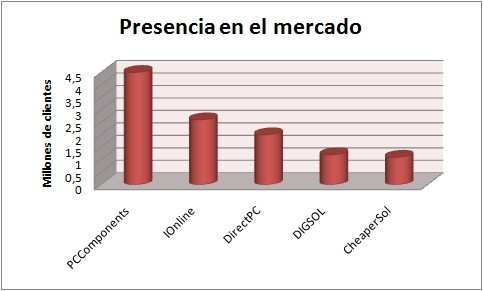
\includegraphics[scale=0.7,keepaspectratio]{./images/presencia}%
\caption{Presencia en el mercado de las empresas}%
\label{fig:presencia}%
\end{figure}

\subsection{ANEXO 2: Organigrama de la empresa DIGSOL} \label{anexo:organigrama}

\begin{spacing}{1.4}
El organigrama mostrado en la Figura \ref{fig:organigrama} ha sido cedido por el Comit� de Direcci�n de la empresa DIGSOL.
\end{spacing}

\begin{figure}[h]
\centering
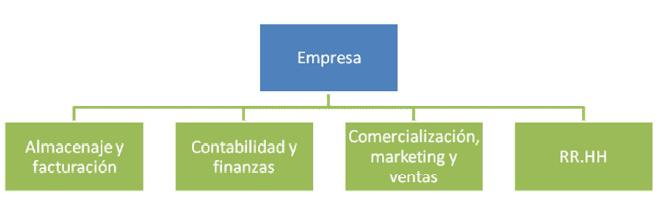
\includegraphics[scale=0.7,keepaspectratio]{./images/organigrama}%
\caption{Organigrama de la empresa DIGSOL}%
\label{fig:organigrama}%
\end{figure}


\subsection{ANEXO 3: Adquisiciones tecnol�gicas} \label{anexo:facturas}

\begin{spacing}{1.4}

Los fragmentos de facturas mostradas en las Figuras \ref{fig:factura} y \ref{fig:facturaAntigua} han sido cedidas por la Direcci�n de la empresa DIGSOL. 

La Figura \ref{fig:facturaAntigua} muestra la adquisici�n que dicha empresa realiz� a mediados del a�o 2008, cuando implant� el servicio de venta Web y actualiz� los equipos de algunos de sus departamentos.

\begin{figure}[ht]
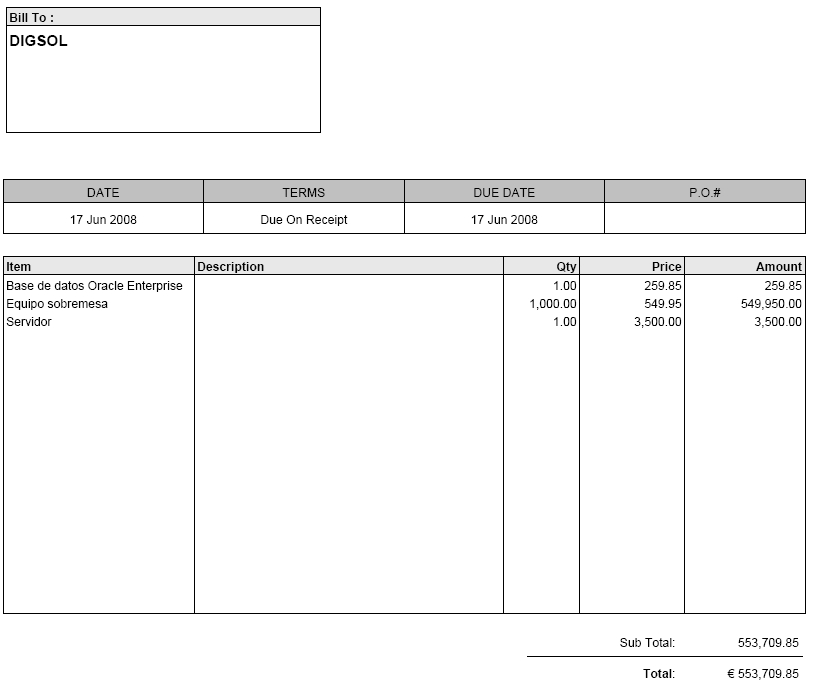
\includegraphics[scale=0.57,keepaspectratio]{./images/facturaAntigua}%
\caption{Fragmento de la factura del 17-Junio-2008}%
\label{fig:facturaAntigua}%
\end{figure}

En la factura de la Figura \ref{fig:factura} se muestra una de las �ltimas adquisiciones que ha realizado la empresa, remarcando gastos que podr�an haberse evitado (en color amarillo) y gastos totalmente innecesarios que no aportan nada de beneficio al negocio (en color rojo). 

\begin{figure}[ht]
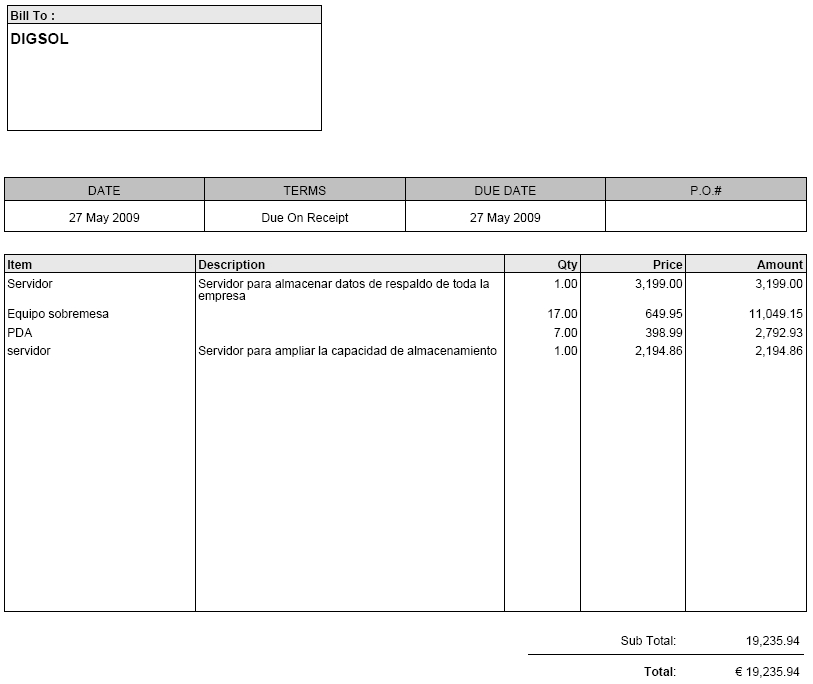
\includegraphics[scale=0.57,keepaspectratio]{./images/factura}%
\caption{Factura del 27-Mayo-2009}%
\label{fig:factura}%
\end{figure}



%El servidor de respaldo es una adquisici�n necesaria, ya que la empresa no lo renovaba desde hace unos 3 o 4 a�os. Sin embargo, la compra de los 17 equipos de sobremesa, destinados al departamento de contabilidad de la sede auditada, es algo innecesario, ya que pr�cticamente la totalidad de equipos se renovaron hace poco m�s de un a�o (coincidiendo con la implantaci�n del sistema Web), tal y como muestra la factura de esa �poca (ver Figura \ref{fig:facturaAntigua}).

%Del mismo modo, adquirir un nuevo servidor para ampliar la capacidad de almacenamiento es, en el momento actual en el que se encuentra la empresa, algo innecsario, pues el servidor que se adquiri� en su dia tiene capacidad suficiente. Podr�a pensarse entonces en qu� es una adquisici�n �til para medio o largo plazo, pero esto no es as�, ya que las tecnolog�as avanzan r�pidamente y en un plazo relativamente corto, existir�n mejores soluciones en el mercado.

%En lo que se refiere a la compra de las PDAs para las personas que integran el comit� de Direcci�n, es un gasto totalmente no justificado e in�til, ya que no se utilizan dichas PDAs para proporcionar valor al negocio. Podr�an aprovecharse para sincronizar los datos de la empresa en las PDAs, atender negocios en ella, etc., pero esto no ocurre as�.


\end{spacing}


\end{document}
